\documentclass[12pt,a4paper]{article}
\usepackage{ucebnice}

\title{Geometrická zobrazení}
\author{Ondřej Škubala}
\date{\today}

\begin{document}

\maketitle
\newpage

% ============================================================
% GEOMETRICKÁ ZOBRAZENÍ
% ============================================================

\section{Geometrická zobrazení}

V dosavadní geometrii jsme většinou zkoumali jednotlivé útvary, jejich strany, úhly, vzdálenosti nebo vzájemnou polohu. Nyní se na rovinu podíváme trochu jiným způsobem: nebudeme sledovat pouze jeden útvar, ale budeme zkoumat, jak lze body a celé útvary v rovině systematicky převádět na jiné body a jiné útvary, přičemž nás bude zajímat zejména to, které vlastnosti se při takovém převodu zachovají a které se naopak mohou změnit.

Takovému předpisu budeme říkat \textbf{geometrické zobrazení}. Může například převést trojúhelník na jeho zrcadlový obraz, posunout jej o několik centimetrů doprava, otočit jej kolem zvoleného bodu nebo jej zvětšit na dvojnásobnou velikost. Přestože výsledné útvary mohou na první pohled vypadat různě, jejich geometrické vlastnosti jsou mezi sebou přesně svázány pravidly použitého zobrazení.

\subsection{Zobrazení bodů a útvarů}

Uvažujme rovinu $\rho$. Geometrické zobrazení budeme chápat jako předpis, který každému bodu $X$ roviny přiřadí právě jeden bod $X'$ téže roviny. Zapisujeme například
\[
    X \mapsto X',
\]
a říkáme, že bod $X$ je \textbf{vzor} a bod $X'$ jeho \textbf{obraz}. Jestliže takto zobrazíme všechny body určitého útvaru $U$, dostaneme jeho obraz $U'$.

\begin{definitionbox}
    \important{Geometrické zobrazení v rovině} je předpis, který bodům roviny přiřazuje body téže roviny. Je-li bodu $X$ přiřazen bod $X'$, zapisujeme
    \[
        X \mapsto X'.
    \]
    Bod $X$ nazýváme \textbf{vzorem} a bod $X'$ jeho \textbf{obrazem}.
\end{definitionbox}

Z podmínky, že každému bodu přiřazujeme právě jeden obraz, plyne především jednoznačnost zobrazení: jakmile známe bod $X$, jeho obraz $X'$ je určen jednoznačně. Obrácený postup však nemusí být možný vždy. Může se totiž stát, že se několik různých bodů zobrazí do téhož bodu, a potom z obrazu nedokážeme jednoznačně určit původní vzor.

\subsubsection*{Prosté a inverzní zobrazení}

Zobrazení nazýváme \textbf{prostým}, jestliže se dva různé body nikdy nezobrazí do téhož bodu. U zobrazení, která jsou současně prostá a zobrazují rovinu na celou rovinu, můžeme směr zobrazování obrátit a ke každému obrazu znovu jednoznačně určit jeho vzor. Takové obrácené zobrazení nazýváme \textbf{inverzním zobrazením}.

\begin{notebox}
    U zobrazení, kterými se budeme zabývat v této kapitole, inverzní zobrazení existuje. Osová a středová souměrnost jsou samy sobě inverzní, opačné posunutí získáme změnou směru posunu, opačné otočení změnou znaménka úhlu a ke stejnolehlosti s koeficientem $\lambda$ je inverzní stejnolehlost s koeficientem $1/\lambda$.
\end{notebox}

Pokud se některý bod při zobrazení nezmění, tedy jestliže $X'=X$, nazýváme jej \textbf{samodružným bodem}. Podobně můžeme mluvit také o samodružné přímce, kružnici nebo obecně o samodružném útvaru; v takovém případě se útvar jako celek zobrazí sám na sebe, i když se jeho jednotlivé body nemusí všechny zobrazit samy na sebe.

\begin{notebox}
    Je důležité rozlišovat dvě situace. Jestliže se každý bod útvaru zobrazí sám na sebe, pak je útvar tvořen pouze samodružnými body. Pokud se však například kružnice při otočení kolem svého středu zobrazí sama na sebe, je jako celek samodružná, avšak většina jejích bodů se přemístí na jiná místa kružnice.
\end{notebox}

\subsection{Shodná a podobná zobrazení}

Geometrických zobrazení lze vytvořit velmi mnoho, pro středoškolskou geometrii jsou však nejdůležitější dvě velké skupiny: \textbf{shodná zobrazení} a \textbf{podobná zobrazení}. Rozdíl mezi nimi spočívá především v tom, co se děje se vzdálenostmi bodů.

Při shodném zobrazení se žádná vzdálenost nemění. Jestliže tedy body $A$, $B$ přejdou na body $A'$, $B'$, potom platí
\[
    |A'B'|=|AB|.
\]
Útvar se může přemístit, otočit nebo zrcadlově převrátit, ale jeho velikost zůstává stejná.

Při podobném zobrazení se všechny vzdálenosti násobí stejným kladným číslem $k$, kterému říkáme \textbf{koeficient podobnosti}. Platí tedy
\[
    |A'B'|=k\,|AB|,
    \qquad k>0.
\]
Pro $k>1$ se všechny délky zvětšují, pro $0<k<1$ se zmenšují a pro $k=1$ se jejich velikost nemění, takže shodné zobrazení je zvláštním případem podobného zobrazení.

\begin{center}
\begin{tikzpicture}[scale=0.82]
    % původní trojúhelník
    \coordinate (A) at (0,0);
    \coordinate (B) at (3.2,0.4);
    \coordinate (C) at (1.1,2.3);
    \draw[very thick] (A)--(B)--(C)--cycle;
    \node[below] at (A) {$A$};
    \node[below] at (B) {$B$};
    \node[above] at (C) {$C$};
    \node at (1.5,-0.8) {původní útvar};

    % shodný obraz
    \coordinate (As) at (5.0,0.3);
    \coordinate (Bs) at (8.2,-0.1);
    \coordinate (Cs) at (7.1,2.2);
    \draw[very thick, tableborder] (As)--(Bs)--(Cs)--cycle;
    \node[below] at (As) {$A'$};
    \node[below] at (Bs) {$B'$};
    \node[above] at (Cs) {$C'$};
    \node[text=tableborder] at (6.6,-0.8) {shodný obraz};

    % podobný obraz
    \coordinate (Ap) at (10.0,-0.2);
    \coordinate (Bp) at (14.5,0.35);
    \coordinate (Cp) at (11.55,3.05);
    \draw[very thick, pastelgreen!55!black] (Ap)--(Bp)--(Cp)--cycle;
    \node[below] at (Ap) {$A''$};
    \node[below] at (Bp) {$B''$};
    \node[above] at (Cp) {$C''$};
    \node[text=pastelgreen!55!black] at (12.2,-0.8) {podobný obraz};
\end{tikzpicture}
\end{center}

\subsection{Shodné a podobné útvary}

Pojmy \emph{shodné zobrazení} a \emph{shodné útvary} spolu úzce souvisejí, nejsou však totožné. Shodné zobrazení je předpis, kterým převádíme body roviny na jejich obrazy, zatímco shodnost dvou útvarů vyjadřuje vztah mezi těmito dvěma útvary.

\begin{definitionbox}
    Dva geometrické útvary nazýváme \important{shodné}, jestliže existuje shodné zobrazení, které jeden z nich zobrazí na druhý.
\end{definitionbox}

Shodné útvary tedy mají stejné odpovídající délky, stejné odpovídající úhly, stejný obvod i stejný obsah. Mohou se však nacházet na jiném místě roviny nebo mohou být vůči sobě zrcadlově převráceny.

\begin{definitionbox}
    Dva geometrické útvary nazýváme \important{podobné}, jestliže existuje podobné zobrazení, které jeden z nich zobrazí na druhý.
\end{definitionbox}

Podobné útvary mají stejné odpovídající úhly a poměry odpovídajících délek jsou konstantní. Jejich velikost však obecně stejná být nemusí. Jestliže je koeficient podobnosti $k$, potom se obvody násobí číslem $k$, zatímco obsahy se násobí číslem $k^2$.

\begin{notebox}
    Každé dva shodné útvary jsou zároveň podobné s koeficientem podobnosti $k=1$, opačné tvrzení však obecně neplatí. Dva trojúhelníky mohou mít stejné úhly a odpovídající strany například v poměru $2:1$; potom jsou podobné, ale nejsou shodné.
\end{notebox}

\subsection{Orientace útvaru}

Při některých zobrazeních se zachová nejen tvar a velikost útvaru, ale také jeho \textbf{orientace}. U trojúhelníku můžeme například sledovat pořadí vrcholů $A$, $B$, $C$. Jestliže je obcházíme proti směru hodinových ručiček a obrazy $A'$, $B'$, $C'$ jsou ve stejném pořadí rovněž proti směru hodinových ručiček, orientace se zachovala. Pokud se pořadí obrátí, orientace se změnila.

Toto rozlišení budeme později používat k dělení shodností i podobností na \textbf{přímé} a \textbf{nepřímé}. Nejprve si však ukážeme konkrétní shodná zobrazení, protože na nich bude význam orientace mnohem lépe vidět.


% ============================================================
% SHODNÁ ZOBRAZENÍ
% ============================================================

\section{Shodná zobrazení}

\subsection{Základní vlastnosti shodných zobrazení}

Shodné zobrazení, někdy také nazývané \textbf{izometrie}, je zobrazení, při kterém se zachovávají všechny vzdálenosti. To znamená, že libovolné dva body roviny mají po zobrazení stejnou vzájemnou vzdálenost jako před ním.

\begin{definitionbox}
    Zobrazení roviny nazýváme \important{shodným zobrazením}, jestliže pro každé dva body $A$, $B$ a jejich obrazy $A'$, $B'$ platí
    \[
        |A'B'|=|AB|.
    \]
\end{definitionbox}

Ze zachování vzdáleností plyne řada dalších důležitých vlastností. Shodné zobrazení zachovává délky úseček, velikosti úhlů, rovnoběžnost a kolmost přímek, obvody i obsahy útvarů. Přímka se zobrazí na přímku, polopřímka na polopřímku, polorovina na polorovinu a kružnice na kružnici se stejným poloměrem. Obrazem dvojice rovnoběžných přímek jsou opět rovnoběžné přímky a obrazem dvojice kolmých přímek jsou opět přímky kolmé.

\begin{center}
\begin{tabular}{|C{5.2cm}|C{8.2cm}|}
    \hline
    \rowcolor{pastelblue!45}
    \textbf{Vzor} & \textbf{Obraz v libovolném shodném zobrazení} \\
    \hline
    úsečka délky $a$ & úsečka délky $a$ \\
    \hline
    úhel $\alpha$ & úhel velikosti $\alpha$ \\
    \hline
    přímka & přímka \\
    \hline
    rovnoběžné přímky & rovnoběžné přímky \\
    \hline
    kružnice o poloměru $r$ & kružnice o poloměru $r$ \\
    \hline
    útvar s obsahem $S$ & útvar s obsahem $S$ \\
    \hline
\end{tabular}
\end{center}

Mezi základní shodná zobrazení v rovině patří \textbf{osová souměrnost}, \textbf{středová souměrnost}, \textbf{posunutí} a \textbf{otočení}.


% ------------------------------------------------------------
% OSOVÁ SOUMĚRNOST
% ------------------------------------------------------------

\subsection{Osová souměrnost}

Osovou souměrnost známe intuitivně například ze zrcadlení. Zvolíme přímku $o$, kterou nazveme \textbf{osou souměrnosti}, a každý bod roviny zobrazíme na bod ležící stejně daleko od této osy, avšak na opačné straně.

\begin{definitionbox}
    \important{Osová souměrnost} s osou $o$ je zobrazení, které bodu $A\notin o$ přiřadí bod $A'$ tak, že přímka $o$ je osou úsečky $AA'$. Každý bod ležící na ose $o$ se zobrazí sám na sebe.
\end{definitionbox}

Jestliže $A\notin o$, potom platí
\[
    AA'\perp o
\]
a průsečík úsečky $AA'$ s osou $o$ je středem této úsečky. Body osy $o$ jsou tedy právě samodružnými body osové souměrnosti.

\begin{figure}[ht]
    \centering
    \begin{tikzpicture}[scale=0.9]
        \draw[very thick] (0,-0.5)--(0,5) node[above] {$o$};

        \coordinate (A) at (-3.5,0.4);
        \coordinate (B) at (-1.5,0.8);
        \coordinate (C) at (-2.8,3.5);
        \coordinate (Ap) at (3.5,0.4);
        \coordinate (Bp) at (1.5,0.8);
        \coordinate (Cp) at (2.8,3.5);

        \draw[very thick, tableborder] (A)--(B)--(C)--cycle;
        \draw[very thick, pastelgreen!60!black] (Ap)--(Bp)--(Cp)--cycle;

        \draw[dashed, gray] (A)--(Ap);
        \draw[dashed, gray] (B)--(Bp);
        \draw[dashed, gray] (C)--(Cp);

        \fill (A) circle (1.6pt) node[left] {$A$};
        \fill (B) circle (1.6pt) node[below] {$B$};
        \fill (C) circle (1.6pt) node[left] {$C$};
        \fill (Ap) circle (1.6pt) node[right] {$A'$};
        \fill (Bp) circle (1.6pt) node[below] {$B'$};
        \fill (Cp) circle (1.6pt) node[right] {$C'$};
    \end{tikzpicture}
    \caption{Osová souměrnost trojúhelníku podle osy $o$.}
\end{figure}

Konstrukce obrazu bodu $A$ je přímočará. Nejprve bodem $A$ vedeme kolmici k ose $o$ a její průsečík s osou označíme $P$. Potom na stejné kolmici na opačné straně od osy sestrojíme bod $A'$ tak, aby platilo
\[
    |PA|=|PA'|.
\]

\begin{examplebox}
    Máme-li zobrazit trojúhelník $ABC$ v osové souměrnosti podle přímky $o$, zobrazíme postupně jeho vrcholy $A$, $B$, $C$ na body $A'$, $B'$, $C'$ a tyto obrazy spojíme. Protože osová souměrnost zachovává vzdálenosti i velikosti úhlů, je trojúhelník $A'B'C'$ shodný s trojúhelníkem $ABC$.
\end{examplebox}

Osová souměrnost mění orientaci. Jestliže byly vrcholy trojúhelníku $A$, $B$, $C$ uspořádány proti směru hodinových ručiček, potom budou jejich obrazy $A'$, $B'$, $C'$ uspořádány po směru hodinových ručiček. Proto je osová souměrnost \textbf{nepřímou shodností}.




\subsubsection*{Samodružné body, přímky a osa souměrnosti útvaru}

Množinu všech samodružných bodů osové souměrnosti tvoří právě její osa $o$. Samodružná však může být i přímka, jejíž všechny body samodružné nejsou. Kromě samotné osy $o$ je totiž samodružná každá přímka kolmá na osu $o$: při zobrazení se sice její body navzájem vymění, ale jako celek zůstane tatáž přímka.

Pokud se celý geometrický útvar v osové souměrnosti zobrazí sám na sebe, nazýváme přímku $o$ \textbf{osou souměrnosti útvaru}. Čtverec má čtyři osy souměrnosti, obdélník, který není čtvercem, má dvě, a obecný rovnoběžník nemusí mít žádnou.

\begin{examplebox}
    Jsou dány dva různé body $A$ a $B$. Chceme určit osu takové osové souměrnosti, která zobrazí $A$ na $B$. Protože osa souměrnosti musí být kolmá k úsečce $AB$ a současně musí procházet jejím středem, je hledanou osou právě \textbf{osa úsečky $AB$}. Z jediné dvojice odpovídajících si bodů tak dokážeme osovou souměrnost jednoznačně určit.
\end{examplebox}

Osová souměrnost je sama sobě inverzní. Provedeme-li tutéž osovou souměrnost dvakrát, každý bod se vrátí na své původní místo.

\subsubsection*{Osová souměrnost jako nástroj optimalizace}

Osová souměrnost není užitečná pouze při zobrazování útvarů. Umožňuje také převést některé úlohy o nejkratší cestě na jednoduchou vlastnost, že nejkratší spojnicí dvou bodů je úsečka.

\begin{examplebox}
    Body $A$ a $B$ leží ve stejné polorovině určené přímkou $p$. Na přímce $p$ hledáme bod $X$ tak, aby součet
    \[
        |AX|+|XB|
    \]
    byl co nejmenší. Zobrazíme bod $B$ v osové souměrnosti podle přímky $p$ na bod $B'$. Pro každý bod $X\in p$ platí $|XB|=|XB'|$, a tedy
    \[
        |AX|+|XB|=|AX|+|XB'|.
    \]
    Nejmenší hodnoty dosáhneme tehdy, když body $A$, $X$, $B'$ leží na jedné přímce. Hledaný bod je proto průsečíkem přímek $AB'$ a $p$.
\end{examplebox}

% ------------------------------------------------------------
% STŘEDOVÁ SOUMĚRNOST
% ------------------------------------------------------------

\subsection{Středová souměrnost}

U středové souměrnosti již nemáme osu, ale jediný pevně zvolený bod $S$, který nazýváme \textbf{středem souměrnosti}. Bod $A$ se zobrazí na bod $A'$ tak, že střed $S$ leží přesně uprostřed úsečky $AA'$.

\begin{definitionbox}
    \important{Středová souměrnost} se středem $S$ je zobrazení, které každému bodu $A\neq S$ přiřadí bod $A'$ tak, že $S$ je středem úsečky $AA'$. Bod $S$ se zobrazí sám na sebe.
\end{definitionbox}

Pro bod $A$ a jeho obraz $A'$ tedy platí
\[
    A,S,A' \text{ leží na jedné přímce}
\]
a současně
\[
    |SA|=|SA'|.
\]
Vektorově můžeme tento vztah zapsat jako
\[
    \overrightarrow{SA'}=-\overrightarrow{SA}.
\]

\begin{figure}[ht]
    \centering
    \begin{tikzpicture}[scale=0.9]
        \coordinate (S) at (0,0);
        \coordinate (A) at (-3.5,-0.8);
        \coordinate (B) at (-1.0,-1.5);
        \coordinate (C) at (-2.2,1.7);
        \coordinate (Ap) at (3.5,0.8);
        \coordinate (Bp) at (1.0,1.5);
        \coordinate (Cp) at (2.2,-1.7);

        \draw[very thick, tableborder] (A)--(B)--(C)--cycle;
        \draw[very thick, pastelgreen!60!black] (Ap)--(Bp)--(Cp)--cycle;
        \draw[dashed, gray] (A)--(Ap);
        \draw[dashed, gray] (B)--(Bp);
        \draw[dashed, gray] (C)--(Cp);

        \fill (S) circle (2pt) node[above right] {$S$};
        \fill (A) circle (1.5pt) node[left] {$A$};
        \fill (B) circle (1.5pt) node[below] {$B$};
        \fill (C) circle (1.5pt) node[above] {$C$};
        \fill (Ap) circle (1.5pt) node[right] {$A'$};
        \fill (Bp) circle (1.5pt) node[above] {$B'$};
        \fill (Cp) circle (1.5pt) node[below] {$C'$};
    \end{tikzpicture}
    \caption{Středová souměrnost se středem $S$.}
\end{figure}

Jediným samodružným bodem netriviální středové souměrnosti je její střed $S$. Přímka procházející středem $S$ se zobrazí sama na sebe, avšak její body se obecně navzájem vymění. Přímka, která středem $S$ neprochází, se zobrazí na přímku s ní rovnoběžnou.

Středová souměrnost je současně zvláštním případem otočení: odpovídá otočení o úhel $180^\circ$ kolem bodu $S$. Z tohoto důvodu zachovává orientaci a patří mezi \textbf{přímé shodnosti}.




\subsubsection*{Obraz přímky a samodružné přímky}

Přímka procházející středem souměrnosti $S$ se zobrazí sama na sebe. Přímka, která bodem $S$ neprochází, se zobrazí na přímku s ní rovnoběžnou. Při konstrukci obrazu přímky proto nemusíme zobrazovat dva libovolné body: stačí zobrazit jeden její bod a tímto obrazem vést rovnoběžku s původní přímkou.

Středová souměrnost je stejně jako osová souměrnost sama sobě inverzní. Pokud bod $A$ přejde na $A'$, pak při téže středové souměrnosti přejde $A'$ zpět na $A$.

\begin{examplebox}
    Ve čtyřúhelníku $ABCD$ se úhlopříčky $AC$ a $BD$ navzájem půlí v bodě $S$. Proto jsou body $A$ a $C$ středově souměrné podle $S$ a stejně tak body $B$ a $D$. Přímka $AB$ se tedy zobrazí na přímku $CD$, takže $AB\parallel CD$, a přímka $BC$ se zobrazí na přímku $AD$, takže $BC\parallel AD$. Čtyřúhelník $ABCD$ je proto rovnoběžník.
\end{examplebox}

% ------------------------------------------------------------
% POSUNUTÍ
% ------------------------------------------------------------

\subsection{Posunutí}

Posunutí, neboli translace, přesouvá všechny body roviny stejným směrem a o stejnou vzdálenost. Abychom dokázali tento pohyb přesně popsat ještě dříve, než začneme systematicky pracovat s vektory, použijeme \textbf{orientovanou úsečku}.

\subsubsection*{Orientovaná úsečka}

U obyčejné úsečky $AB$ nerozlišujeme, který z bodů $A$, $B$ je první. U orientované úsečky však jeden bod označíme jako počáteční a druhý jako koncový, takže orientované úsečky $\overrightarrow{AB}$ a $\overrightarrow{BA}$ nejsou stejné. Orientovaná úsečka tak určuje zároveň délku i směr posunutí.

\begin{notebox}
    Orientovaná úsečka velmi úzce souvisí s vektorem. Rozdíl spočívá především v tom, že u orientované úsečky známe také její konkrétní umístění v rovině, zatímco stejný vektor můžeme v rovině zakreslit na mnoha různých místech.
\end{notebox}

\begin{definitionbox}
    Je dána orientovaná úsečka $\overrightarrow{AB}$. \important{Posunutí} určené touto orientovanou úsečkou je shodné zobrazení, které každému bodu $X$ přiřadí bod $X'$ tak, že orientované úsečky $\overrightarrow{XX'}$ a $\overrightarrow{AB}$ mají stejnou délku a stejný směr. Symbolicky můžeme psát
    \[
        T(\overrightarrow{AB}) : X\mapsto X'.
    \]
\end{definitionbox}

Později, až budeme pracovat s vektory, lze tutéž definici stručně zapsat vztahem
\[
    \overrightarrow{XX'}=\vec v,
\]
kde $\vec v=\overrightarrow{AB}$ je vektor posunutí.

\begin{figure}[ht]
    \centering
    \begin{tikzpicture}[scale=0.9]
        \coordinate (A) at (0,0);
        \coordinate (B) at (3,0.4);
        \coordinate (C) at (1.2,2.2);
        \coordinate (Ap) at (5,1.0);
        \coordinate (Bp) at (8,1.4);
        \coordinate (Cp) at (6.2,3.2);

        \draw[very thick, tableborder] (A)--(B)--(C)--cycle;
        \draw[very thick, pastelgreen!60!black] (Ap)--(Bp)--(Cp)--cycle;

        \draw[->, very thick] (A)--(Ap);
        \draw[->, thick, gray] (B)--(Bp);
        \draw[->, thick, gray] (C)--(Cp);
        \node[above] at (2.7,0.55) {$\overrightarrow{AA'}$};

        \node[below] at (A) {$A$};
        \node[below] at (B) {$B$};
        \node[above] at (C) {$C$};
        \node[below] at (Ap) {$A'$};
        \node[below] at (Bp) {$B'$};
        \node[above] at (Cp) {$C'$};
    \end{tikzpicture}
    \caption{Posunutí trojúhelníku: všechny body se přesouvají stejným směrem a o stejnou vzdálenost.}
\end{figure}

Je-li posunutí nenulové, nemá žádný samodružný bod. Obrazem každé přímky je přímka s ní rovnoběžná; jestliže je původní přímka rovnoběžná se směrem posunutí, zobrazí se jako celek sama na sebe. Inverzním zobrazením k $T(\overrightarrow{AB})$ je posunutí v opačném směru,
\[
    T(\overrightarrow{BA}).
\]
Posunutí zachovává orientaci, a proto je \textbf{přímou shodností}.

\begin{examplebox}
    Jsou dány dvě různoběžné přímky $a$, $b$ a úsečka $KL$. Hledáme úsečku $AB$, která je s $KL$ rovnoběžná a shodná, přičemž $A\in a$ a $B\in b$. Bod $B$ musí být obrazem bodu $A$ buď v posunutí $T(\overrightarrow{KL})$, nebo v opačném posunutí $T(\overrightarrow{LK})$. Zobrazíme proto celou přímku $a$ v obou těchto posunutích. Její průsečíky s přímkou $b$ určují možné polohy bodu $B$ a zpětným posunutím získáme odpovídající body $A$.
\end{examplebox}

% ------------------------------------------------------------
% OTOČENÍ
% ------------------------------------------------------------

\subsection{Otočení}

Při otočení zůstává jeden bod roviny pevný a ostatní body se pohybují po kružnicích se středem v tomto pevném bodě. Abychom však mohli jednoznačně určit nejen velikost, ale také směr otočení, potřebujeme nejprve pojem \textbf{orientovaného úhlu}.

\subsubsection*{Orientovaný úhel}

Běžný úhel chápeme jako část roviny sevřenou dvěma polopřímkami, takový popis však při otáčení nestačí. Potřebujeme rozlišit, které rameno je počáteční, které koncové a kterým směrem se z jednoho do druhého otáčíme. Orientovaný úhel proto tvoří uspořádaná dvojice polopřímek se společným počátkem.

Za \textbf{kladný směr} otáčení považujeme směr proti chodu hodinových ručiček a za \textbf{záporný směr} směr po chodu hodinových ručiček. Základní velikost orientovaného úhlu volíme z intervalu
\[
    \langle 0^\circ;360^\circ),
\]
případně v obloukové míře z intervalu $\langle0;2\pi)$. Tentýž orientovaný úhel však můžeme popsat nekonečně mnoha hodnotami, které se liší o celočíselný násobek $360^\circ$.

\begin{examplebox}
    Jestliže se počáteční rameno musí do koncového ramena otočit o $90^\circ$ po směru hodinových ručiček, můžeme velikost orientovaného úhlu zapsat jako $-90^\circ$. Jeho základní velikost je však $270^\circ$.
\end{examplebox}

\begin{definitionbox}
    Je dán bod $S$ a orientovaný úhel o velikosti $\varphi$. \important{Otočení} se středem $S$ a úhlem $\varphi$ je shodné zobrazení, které bodu $A\neq S$ přiřadí bod $A'$ tak, že
    \[
        |SA'|=|SA|
    \]
    a orientovaný úhel $\angle ASA'$ má velikost $\varphi$. Bod $S$ se zobrazí sám na sebe.
\end{definitionbox}

\begin{figure}[ht]
    \centering
    \begin{tikzpicture}[scale=0.9]
        \coordinate (S) at (0,0);
        \coordinate (A) at (4,0);
        \coordinate (B) at (5,1.2);
        \coordinate (C) at (3.3,2.1);
        \coordinate (Ap) at (2.0,3.464);
        \coordinate (Bp) at (1.46,4.93);
        \coordinate (Cp) at (-0.17,3.91);

        \draw[very thick, tableborder] (A)--(B)--(C)--cycle;
        \draw[very thick, pastelgreen!60!black] (Ap)--(Bp)--(Cp)--cycle;

        \draw[dashed, gray] (S)--(A);
        \draw[dashed, gray] (S)--(Ap);
        \draw[->, thick] (1.4,0) arc (0:60:1.4);
        \node at (1.55,0.95) {$\varphi$};

        \fill (S) circle (2pt) node[below left] {$S$};
        \node[below] at (A) {$A$};
        \node[below right] at (B) {$B$};
        \node[above] at (C) {$C$};
        \node[above left] at (Ap) {$A'$};
        \node[above] at (Bp) {$B'$};
        \node[left] at (Cp) {$C'$};
    \end{tikzpicture}
    \caption{Otočení trojúhelníku kolem bodu $S$ o úhel $\varphi$.}
\end{figure}

Jestliže $\varphi$ není celočíselným násobkem $360^\circ$, je jediným samodružným bodem otočení jeho střed $S$. Pro úhel $\varphi=180^\circ$ dostáváme středovou souměrnost a pro $\varphi=0^\circ$ identické zobrazení. Inverzním zobrazením k otočení o úhel $\varphi$ je otočení kolem téhož středu o úhel $-\varphi$.

Obraz přímky můžeme vždy určit z obrazů dvou jejích bodů. Prakticky výhodnější postup dostaneme tehdy, když ze středu otočení $S$ spustíme kolmici na zobrazovanou přímku $p$ a její patu označíme $P$. Po otočení bodu $P$ na $P'$ bude obraz přímky $p'$ kolmý na $SP'$ a bude procházet bodem $P'$.

Otočení zachovává orientaci, a proto je vždy \textbf{přímou shodností}.

\begin{examplebox}
    Jsou dány dvě rovnoběžné přímky $a$, $b$ a mimo ně bod $C$. Hledáme rovnostranný trojúhelník $ABC$ tak, aby $A\in a$ a $B\in b$. Protože v rovnostranném trojúhelníku platí $|CA|=|CB|$ a $|\angle ACB|=60^\circ$, lze bod $A$ zobrazit na bod $B$ otočením kolem $C$ o $60^\circ$ nebo o $-60^\circ$. Zobrazíme tedy přímku $a$ v obou otočeních a její obrazy protneme s přímkou $b$. Tak získáme možné body $B$ a zpětným otočením odpovídající vrcholy $A$.
\end{examplebox}

% ------------------------------------------------------------
% PŘÍMÁ A NEPŘÍMÁ SHODNOST
% ------------------------------------------------------------

\subsection{Přímá a nepřímá shodnost}

Nyní již můžeme přesněji vysvětlit rozdělení shodných zobrazení podle orientace. Pokud se orientace každého útvaru při zobrazení zachová, hovoříme o přímé shodnosti. Pokud se orientace obrátí, jde o nepřímou shodnost.

\begin{definitionbox}
    \important{Přímá shodnost} je shodné zobrazení, které zachovává orientaci útvarů. \important{Nepřímá shodnost} je shodné zobrazení, které orientaci obrací.
\end{definitionbox}

\begin{center}
\begin{tabular}{|C{4.7cm}|C{4.7cm}|C{4.0cm}|}
    \hline
    \rowcolor{pastelblue!45}
    \textbf{Zobrazení} & \textbf{Orientace} & \textbf{Typ shodnosti} \\
    \hline
    posunutí & zachována & přímá \\
    \hline
    otočení & zachována & přímá \\
    \hline
    středová souměrnost & zachována & přímá \\
    \hline
    osová souměrnost & obrácena & nepřímá \\
    \hline
\end{tabular}
\end{center}

\begin{notebox}
    Existují i další shodná zobrazení, která lze získat skládáním těch základních. Například složením osové souměrnosti s vhodným posunutím ve směru osy vzniká \textbf{posunutá osová souměrnost}. Pro základní přehled nám však postačí čtyři zobrazení uvedená výše.
\end{notebox}

Je užitečné si uvědomit, že složením dvou nepřímých shodností vzniká přímá shodnost. Například dvě osové souměrnosti podle rovnoběžných os dávají posunutí, zatímco dvě osové souměrnosti podle různoběžných os dávají otočení. Tato skutečnost ukazuje, že jednotlivé typy shodných zobrazení nejsou izolované, ale tvoří vzájemně propojený systém.

\subsubsection*{Skládání osových souměrností}

Skládání dvou osových souměrností poskytuje velmi názorné propojení mezi jednotlivými shodnostmi. Jsou-li osy rovnoběžné, výsledkem je posunutí kolmé na obě osy; velikost posunutí je dvojnásobkem vzdálenosti os. Jsou-li osy různoběžné, výsledkem je otočení kolem jejich průsečíku; úhel otočení je dvojnásobkem orientovaného úhlu mezi osami. Tím lze vysvětlit, proč jsou posunutí i otočení přímými shodnostmi: vznikají složením dvou nepřímých shodností.



% ============================================================
% PODOBNÁ ZOBRAZENÍ
% ============================================================

\section{Podobná zobrazení}

\subsection{Základní vlastnosti podobných zobrazení}

U podobného zobrazení již nemusí zůstat zachována samotná délka úsečky, zachovává se však její poměr vůči ostatním délkám. Všechny vzdálenosti jsou totiž násobeny stejným kladným číslem $k$.

\begin{definitionbox}
    Zobrazení roviny nazýváme \important{podobným zobrazením} s koeficientem podobnosti $k>0$, jestliže pro každé dva body $A$, $B$ a jejich obrazy $A'$, $B'$ platí
    \[
        |A'B'|=k\,|AB|.
    \]
\end{definitionbox}

Koeficient podobnosti určuje změnu měřítka. Pro
\[
    k>1
\]
se délky zvětšují, pro
\[
    0<k<1
\]
se zmenšují a pro
\[
    k=1
\]
se nemění, takže dostáváme shodné zobrazení.

Podobné zobrazení zachovává velikosti úhlů, rovnoběžnost a kolmost přímek i poměry délek. Přímky se zobrazují na přímky a kružnice na kružnice. Délky se násobí číslem $k$, obvody rovněž číslem $k$, ale obsahy se násobí číslem $k^2$.

\begin{center}
\begin{tikzpicture}[scale=0.85]
    \coordinate (A) at (0,0);
    \coordinate (B) at (3,0.4);
    \coordinate (C) at (1.0,2.2);
    \coordinate (Ap) at (6,0);
    \coordinate (Bp) at (11.1,0.68);
    \coordinate (Cp) at (7.7,3.74);

    \draw[very thick, tableborder] (A)--(B)--(C)--cycle;
    \draw[very thick, pastelgreen!60!black] (Ap)--(Bp)--(Cp)--cycle;

    \node[below] at (A) {$A$};
    \node[below] at (B) {$B$};
    \node[above] at (C) {$C$};
    \node[below] at (Ap) {$A'$};
    \node[below] at (Bp) {$B'$};
    \node[above] at (Cp) {$C'$};

    \node at (1.5,-0.8) {vzor};
    \node[text=pastelgreen!60!black] at (8.5,-0.8) {obraz pro $k=1{,}7$};
\end{tikzpicture}
\end{center}

\begin{examplebox}
    Jestliže podobné zobrazení s koeficientem $k=3$ zobrazí úsečku délky $4\,\mathrm{cm}$, bude mít její obraz délku
    \[
        3\cdot4=12\,\mathrm{cm}.
    \]
    Má-li původní obrazec obsah $5\,\mathrm{cm}^2$, bude obsah jeho obrazu
    \[
        3^2\cdot5=45\,\mathrm{cm}^2.
    \]
    Právě rozdíl mezi násobením délek číslem $k$ a obsahů číslem $k^2$ je při práci s podobnými útvary velmi důležitý.
\end{examplebox}


% ------------------------------------------------------------
% PŘÍMÁ A NEPŘÍMÁ PODOBNOST
% ------------------------------------------------------------

\subsection{Přímá a nepřímá podobnost}

Stejně jako shodná zobrazení můžeme i podobná zobrazení rozdělit podle toho, zda zachovávají orientaci útvarů.

\begin{definitionbox}
    \important{Přímá podobnost} je podobné zobrazení, které zachovává orientaci. \important{Nepřímá podobnost} je podobné zobrazení, které orientaci obrací.
\end{definitionbox}

Přímou podobnost můžeme intuitivně chápat jako změnu měřítka spojenou případně s posunutím nebo otočením, zatímco nepřímá podobnost navíc obsahuje zrcadlové převrácení. Samotná stejnolehlost, kterou budeme studovat v následující části, je přímou podobností, a to i tehdy, když má záporný koeficient.

\begin{notebox}
    Záporný koeficient stejnolehlosti neznamená nepřímou podobnost. Záporné znaménko pouze určuje, že obraz bodu leží na opačné polopřímce vzhledem ke středu stejnolehlosti. Orientace útvaru se přitom v rovině zachová.
\end{notebox}


% ------------------------------------------------------------
% STEJNOLEHLOST
% ------------------------------------------------------------

\subsection{Stejnolehlost}

Stejnolehlost, neboli homotetie, je základním příkladem podobného zobrazení. Je určena jedním bodem $S$, který nazýváme \textbf{středem stejnolehlosti}, a nenulovým reálným číslem $\lambda$, které nazýváme \textbf{koeficientem stejnolehlosti}.

\begin{definitionbox}
    \important{Stejnolehlost} se středem $S$ a koeficientem $\lambda\neq0$ je zobrazení, které každému bodu $A$ přiřadí bod $A'$ tak, že
    \[
        \overrightarrow{SA'}=\lambda\,\overrightarrow{SA}.
    \]
\end{definitionbox}

Koeficient $\lambda$ nese dvě informace zároveň. Jeho absolutní hodnota $|\lambda|$ určuje, kolikrát se vzdálenosti od středu zvětší nebo zmenší, zatímco znaménko určuje, na které straně středu $S$ bude obraz ležet.

Pro $\lambda>0$ leží body $A$ a $A'$ na stejné polopřímce se začátkem $S$. Pro $\lambda<0$ leží na opačných polopřímkách. Ve všech případech platí
\[
    |SA'|=|\lambda|\,|SA|.
\]
Koeficient podobnosti odpovídající této stejnolehlosti je proto
\[
    k=|\lambda|.
\]

\subsubsection*{Kladný koeficient stejnolehlosti}

Jestliže je $\lambda>0$, zachovává se poloha bodů na stejných polopřímkách vycházejících ze středu $S$. Pro $\lambda>1$ se útvar vzhledem ke středu zvětšuje, zatímco pro $0<\lambda<1$ se zmenšuje.

\begin{figure}[ht]
    \centering
    \begin{tikzpicture}[scale=0.8]
        \coordinate (S) at (0,0);
        \coordinate (A) at (2,0.4);
        \coordinate (B) at (3.2,0.8);
        \coordinate (C) at (2.2,2.0);
        \coordinate (Ap) at (4,0.8);
        \coordinate (Bp) at (6.4,1.6);
        \coordinate (Cp) at (4.4,4.0);

        \draw[dashed, gray] (S)--(6.9,1.75);
        \draw[dashed, gray] (S)--(4.8,4.35);
        \draw[dashed, gray] (S)--(4.5,0.9);

        \draw[very thick, tableborder] (A)--(B)--(C)--cycle;
        \draw[very thick, pastelgreen!60!black] (Ap)--(Bp)--(Cp)--cycle;

        \fill (S) circle (2pt) node[below left] {$S$};
        \node[below] at (A) {$A$};
        \node[below] at (B) {$B$};
        \node[above] at (C) {$C$};
        \node[below] at (Ap) {$A'$};
        \node[right] at (Bp) {$B'$};
        \node[above] at (Cp) {$C'$};
        \node at (5.9,3.5) {$\lambda=2$};
    \end{tikzpicture}
    \caption{Stejnolehlost se středem $S$ a kladným koeficientem $\lambda=2$.}
\end{figure}

\subsubsection*{Záporný koeficient stejnolehlosti}

Pro $\lambda<0$ leží obraz bodu na opačné polopřímce vzhledem ke středu $S$. Vizuálně tak zobrazení připomíná kombinaci středové souměrnosti a změny měřítka.

\begin{figure}[ht]
    \centering
    \begin{tikzpicture}[scale=0.78]
        \coordinate (S) at (0,0);
        \coordinate (A) at (-2.0,-0.5);
        \coordinate (B) at (-3.0,-1.1);
        \coordinate (C) at (-2.2,1.6);
        \coordinate (Ap) at (3.0,0.75);
        \coordinate (Bp) at (4.5,1.65);
        \coordinate (Cp) at (3.3,-2.4);

        \draw[dashed, gray] (B)--(Bp);
        \draw[dashed, gray] (C)--(Cp);
        \draw[dashed, gray] (A)--(Ap);
        \draw[very thick, tableborder] (A)--(B)--(C)--cycle;
        \draw[very thick, pastelgreen!60!black] (Ap)--(Bp)--(Cp)--cycle;

        \fill (S) circle (2pt) node[above left] {$S$};
        \node[left] at (A) {$A$};
        \node[left] at (B) {$B$};
        \node[above] at (C) {$C$};
        \node[right] at (Ap) {$A'$};
        \node[right] at (Bp) {$B'$};
        \node[below] at (Cp) {$C'$};
        \node at (5.6,-1.8) {$\lambda=-1{,}5$};
    \end{tikzpicture}
    \caption{Stejnolehlost se záporným koeficientem $\lambda=-1{,}5$.}
\end{figure}

\subsubsection*{Zvláštní hodnoty koeficientu}

Některé hodnoty $\lambda$ vedou ke známým zobrazením. Pro
\[
    \lambda=1
\]
dostáváme identické zobrazení, protože každý bod zůstává na svém místě. Pro
\[
    \lambda=-1
\]
dostáváme středovou souměrnost se středem $S$. Hodnota $\lambda=0$ se při definici stejnolehlosti nepřipouští, protože by se všechny body zobrazily do jediného bodu $S$ a takové zobrazení by již nebylo podobným zobrazením roviny.

\subsubsection*{Vlastnosti stejnolehlosti}

Stejnolehlost zachovává velikosti úhlů, rovnoběžnost a kolmost. Délky se násobí číslem $|\lambda|$, obvody také číslem $|\lambda|$ a obsahy číslem $\lambda^2$.

Je-li přímka $p$ vedena středem stejnolehlosti $S$, zobrazí se sama na sebe. Jestliže středem $S$ neprochází, zobrazí se na přímku $p'$ rovnoběžnou s $p$. Kružnice se zobrazí na kružnici, přičemž její poloměr se násobí číslem $|\lambda|$.

\begin{center}
\begin{tabular}{|C{5.2cm}|C{8.2cm}|}
    \hline
    \rowcolor{pastelblue!45}
    \textbf{Vlastnost} & \textbf{Obraz ve stejnolehlosti} \\
    \hline
    délka $a$ & $a'=|\lambda|a$ \\
    \hline
    úhel $\alpha$ & $\alpha'=\alpha$ \\
    \hline
    obsah $S$ & $S'=\lambda^2S$ \\
    \hline
    přímka procházející středem & tatáž přímka \\
    \hline
    přímka neprocházející středem & rovnoběžná přímka \\
    \hline
    kružnice o poloměru $r$ & kružnice o poloměru $r'=|\lambda|r$ \\
    \hline
\end{tabular}
\end{center}

\subsubsection*{Konstrukce obrazu ve stejnolehlosti}

Chceme-li sestrojit obraz bodu $A$ ve stejnolehlosti se středem $S$ a koeficientem $\lambda$, nejprve vedeme přímku $SA$. Potom na této přímce určíme bod $A'$ tak, aby platilo
\[
    |SA'|=|\lambda|\,|SA|.
\]
Při $\lambda>0$ leží $A'$ na stejné polopřímce $SA$, při $\lambda<0$ na opačné polopřímce. Obraz mnohoúhelníku získáme zobrazením jednotlivých vrcholů a jejich následným spojením ve stejném pořadí.

\begin{examplebox}
    Je dán trojúhelník $ABC$, střed stejnolehlosti $S$ a koeficient $\lambda=-2$. Pro každý vrchol vedeme přímku spojující tento vrchol se středem $S$. Obrazy $A'$, $B'$, $C'$ leží na opačných polopřímkách než původní vrcholy a jejich vzdálenosti od středu jsou dvojnásobné:
    \[
        |SA'|=2|SA|,\qquad
        |SB'|=2|SB|,\qquad
        |SC'|=2|SC|.
    \]
    Trojúhelník $A'B'C'$ je s trojúhelníkem $ABC$ podobný s koeficientem podobnosti $k=2$.
\end{examplebox}




\subsubsection*{Jak určit střed stejnolehlosti}

Jestliže známe útvar i jeho obraz ve stejnolehlosti, leží střed stejnolehlosti na každé přímce spojující bod se svým obrazem. Máme-li tedy například dvě dvojice odpovídajících si bodů $A,A'$ a $B,B'$, dostaneme střed jako průsečík
\[
    S=AA'\cap BB',
\]
pokud se tyto přímky protínají. Stejná vlastnost vysvětluje, proč jsou odpovídající si strany stejnolehlých mnohoúhelníků rovnoběžné.

\subsubsection*{Konstrukce bez měření délky}

U koeficientů, jako je například $\lambda=\frac13$ nebo $\lambda=-\frac34$, není vhodné potřebné vzdálenosti pouze odměřovat pravítkem. Přesnější konstrukci získáme pomocí podobnosti trojúhelníků a dělení úsečky v daném poměru. Z bodu $S$ vedeme pomocnou polopřímku, na ní vyznačíme potřebný počet stejných dílků a pomocí rovnoběžek přeneseme příslušný poměr na přímku $SA$.

\begin{examplebox}
    Jsou dány body $S$, $A$, $A'$ tak, že $A'$ je obrazem bodu $A$ v neznámé stejnolehlosti se středem $S$. Chceme bez použití měřítka sestrojit obraz $B'$ dalšího bodu $B$. Spojíme $A$ s $B$. Bod $B'$ musí ležet na přímce $SB$ a současně na přímce vedené bodem $A'$ rovnoběžně s $AB$. Průsečík těchto dvou přímek je hledaný bod $B'$. Konstrukce využívá pouze skutečnosti, že trojúhelníky $SAB$ a $SA'B'$ jsou podobné.
\end{examplebox}

Inverzní zobrazení ke stejnolehlosti $H(S;\lambda)$ je stejnolehlost se stejným středem a koeficientem
\[
    \frac{1}{\lambda}.
\]

% ============================================================
% VZTAHY MEZI ZOBRAZENÍMI
% ============================================================

\section{Vztahy mezi základními zobrazeními}

Jednotlivá geometrická zobrazení není vhodné chápat jako několik navzájem nesouvisejících konstrukčních postupů. Ve skutečnosti mezi nimi existují poměrně těsné vztahy a některá zobrazení jsou pouze zvláštními případy obecnějších zobrazení.

Shodná zobrazení jsou podobná zobrazení s koeficientem podobnosti $k=1$. Středová souměrnost je otočení o $180^\circ$ a současně stejnolehlost s koeficientem $\lambda=-1$. Identita je posunutí o nulový vektor, otočení o $0^\circ$ i stejnolehlost s koeficientem $\lambda=1$.

\begin{center}
\begin{tabular}{|C{4.0cm}|C{2.6cm}|C{3.2cm}|C{3.7cm}|}
    \hline
    \rowcolor{pastelblue!45}
    \textbf{Zobrazení} & \textbf{Shodné?} & \textbf{Orientace} & \textbf{Samodružné body} \\
    \hline
    osová souměrnost & ano & obrácená & všechny body osy \\
    \hline
    středová souměrnost & ano & zachována & střed $S$ \\
    \hline
    posunutí $\vec v\neq\vec0$ & ano & zachována & žádné \\
    \hline
    otočení $\varphi\not\equiv0^\circ$ & ano & zachována & střed $S$ \\
    \hline
    stejnolehlost $\lambda\neq1$ & obecně ne & zachována & střed $S$ \\
    \hline
\end{tabular}
\end{center}

\begin{notebox}
    Z hlediska podobnosti je důležité rozlišovat koeficient stejnolehlosti $\lambda$ od koeficientu podobnosti $k$. Koeficient $\lambda$ může být kladný i záporný, protože jeho znaménko určuje polohu obrazu vzhledem ke středu. Koeficient podobnosti je naproti tomu vždy kladný a pro stejnolehlost platí $k=|\lambda|$.
\end{notebox}



% ============================================================
% KONSTRUKČNÍ ÚLOHY
% ============================================================

\section{Konstrukční úlohy}

Geometrická zobrazení nejsou pouze způsobem, jak vytvořit obraz již známého útvaru. V konstrukčních úlohách mohou propojit informace, které jsou samostatně příliš slabé, nebo umožnit nejprve sestrojit jednodušší pomocný útvar a teprve potom jej přemístit do požadované polohy. V praxi se proto velmi často setkáme se dvěma základními myšlenkami.

\subsection{Spojovací úlohy}

Ve \textbf{spojovací úloze} hledáme dva body, o nichž známe vždy jen část informace, například že jeden leží na přímce a druhý na kružnici. Pokud mezi těmito body rozpoznáme vztah popsaný některým geometrickým zobrazením, můžeme zobrazit celou množinu možných poloh jednoho bodu a její průsečík s množinou možných poloh druhého bodu již určí konkrétní řešení.

Tento princip jsme použili například při hledání úsečky $AB$ rovnoběžné a shodné s danou úsečkou $KL$, jejíž krajní body musí ležet na dvou daných přímkách. Posunutí převede informaci $A\in a$ na informaci o poloze bodu $B$, a dvě původně neúplné podmínky se tak spojí v jednu konstrukci.

\subsection{Dokončovací úlohy}

V \textbf{dokončovací úloze} je obtížné splnit všechny podmínky současně. Nejprve proto sestrojíme útvar, který splňuje pouze část zadání, ale jehož konstrukce je jednoduchá. Potom využijeme vhodné shodné nebo podobné zobrazení a celý pomocný útvar přesuneme, otočíme nebo zvětšíme tak, aby splnil i zbývající podmínku.

\begin{notebox}
    Při řešení konstrukčních úloh je užitečné položit si dvě otázky: \emph{Hledám dva body, o kterých mám jen neúplné informace?} Pak může pomoci spojovací postup. Nebo \emph{umím snadno sestrojit téměř správný útvar, kterému chybí jen jedna podmínka?} Pak bývá účinnější dokončovací postup.
\end{notebox}

\begin{examplebox}
    Typickým dokončovacím příkladem je hledání kružnice, která se má dotýkat dvou rovnoběžných přímek a současně procházet zadaným bodem $M$. Nejprve snadno sestrojíme libovolnou kružnici dotýkající se obou rovnoběžek. Potom ji posunujeme ve směru rovnoběžek tak, aby některý její bod přešel právě do bodu $M$. Tím zachováme oba dotyky a doplníme poslední chybějící podmínku.
\end{examplebox}

% ============================================================
% SHRNUTÍ
% ============================================================

\section{Shrnutí}

Geometrické zobrazení přiřazuje bodům roviny jejich obrazy. Podle toho, jak se při zobrazení mění vzdálenosti, rozlišujeme především zobrazení shodná a podobná. Shodná zobrazení zachovávají všechny vzdálenosti, zatímco podobná zobrazení násobí všechny vzdálenosti stejným kladným koeficientem $k$.

Mezi základní shodná zobrazení patří osová souměrnost, středová souměrnost, posunutí a otočení. Posunutí, otočení a středová souměrnost zachovávají orientaci, a jsou tedy přímými shodnostmi, zatímco osová souměrnost orientaci obrací a je nepřímou shodností.

Stejnolehlost je základním podobným zobrazením určeným středem $S$ a nenulovým koeficientem $\lambda$. Pro délky používáme koeficient podobnosti $k=|\lambda|$, zatímco znaménko $\lambda$ určuje, zda leží obraz bodu na stejné, nebo na opačné polopřímce vzhledem ke středu stejnolehlosti.


U všech základních zobrazení v této kapitole existuje také zobrazení inverzní. Osová a středová souměrnost jsou samy sobě inverzní, u posunutí obrátíme směr, u otočení změníme znaménko úhlu a u stejnolehlosti nahradíme koeficient $\lambda$ číslem $1/\lambda$.

\begin{center}
\begin{tabular}{|C{4.1cm}|C{4.4cm}|C{5.0cm}|}
    \hline
    \rowcolor{pastelblue!45}
    \textbf{Pojem} & \textbf{Co se děje s délkami} & \textbf{Hlavní myšlenka} \\
    \hline
    shodné zobrazení & délky se nemění & zachování velikosti i tvaru \\
    \hline
    podobné zobrazení & délky se násobí $k>0$ & zachování tvaru a změna měřítka \\
    \hline
    přímé zobrazení & --- & zachovává orientaci \\
    \hline
    nepřímé zobrazení & --- & obrací orientaci \\
    \hline
    stejnolehlost & délky se násobí $|\lambda|$ & zvětšení či zmenšení vzhledem ke středu \\
    \hline
\end{tabular}
\end{center}




% -----------------------------------------------------------------
% ---------------------- P Ř Í K L A D Y --------------------------
% -----------------------------------------------------------------

\exercisepart

% =========================
% ÚLOHA 1 – Základní úlohy na stejnolehlost
% =========================

\setcounter{section}{1}

\begin{exercise}[Základní úlohy na stejnolehlost]

    Ve všech následujících úlohách je dán střed stejnolehlosti $S$ a příslušné body nebo útvary leží v rovině.
    Sestrojte požadované obrazy.

    \begin{tasks}(2)

        \task Jsou dány body $A$, $B$, $C$. Sestrojte jejich obrazy ve stejnolehlosti $H(S;2)$.

        \task Jsou dány body $K$, $L$, $M$. Sestrojte jejich obrazy ve stejnolehlosti $H(S;\tfrac12)$.

        \task Je dána úsečka $AB$. Sestrojte její obraz ve stejnolehlosti $H(S;-1)$.

        \task Je dán trojúhelník $ABC$. Sestrojte jeho obraz ve stejnolehlosti $H(S;-\tfrac32)$.

        \task Je dán čtyřúhelník $ABCD$. Sestrojte jeho obraz ve stejnolehlosti $H(S;\tfrac23)$.

        \task Je dána kružnice $k(O;r)$. Sestrojte její obraz ve stejnolehlosti $H(S;2)$.

        \task Je dána přímka $p$, přičemž $S\notin p$. Sestrojte její obraz ve stejnolehlosti $H(S;\tfrac32)$.

        \task Je dána přímka $q$, přičemž $S\in q$. Sestrojte její obraz ve stejnolehlosti $H(S;-2)$.

    \end{tasks}

\end{exercise}


% =========================
% ÚLOHA 2 – Obraz trojúhelníku ve stejnolehlosti
% =========================

\begin{exercise}[Sestrojte obraz trojúhelníku ve stejnolehlosti]

    Je dán trojúhelník $ABC$, pro který platí $a=4\,\mathrm{cm}$, $b=3\,\mathrm{cm}$, $c=5\,\mathrm{cm}$.
    Vně trojúhelníku leží bod $S$ tak, že $|AS|=3\,\mathrm{cm}$ a $|CS|=4\,\mathrm{cm}$.
    Narýsujte obraz trojúhelníku $ABC$ ve stejnolehlosti se středem $S$ a koeficientem:

    \begin{tasks}(2)

        \task $\kappa=\tfrac32$

        \task $\kappa=\tfrac13$

        \task $\kappa=-\tfrac12$

        \task $\kappa=-1$

    \end{tasks}

\end{exercise}


% =========================
% ÚLOHA 3 – Obraz čtverce ve stejnolehlosti
% =========================

\begin{exercise}[Sestrojte obraz čtverce ve stejnolehlosti]

    Je dán čtverec $KLMN$ o straně délky $a=4\,\mathrm{cm}$.
    Označte $S$ střed čtverce a sestrojte obraz čtverce ve stejnolehlosti se středem $S$ a koeficientem:

    \begin{tasks}(2)

        \task $\kappa=\tfrac12$

        \task $\kappa=2$

        \task $\kappa=-\tfrac34$

        \task $\kappa=-2$

    \end{tasks}

\end{exercise}


% =========================
% ÚLOHA 4 – Obraz trojúhelníku se středem v těžišti
% =========================

\begin{exercise}[Sestrojte obraz trojúhelníku se středem stejnolehlosti v těžišti]

    Sestrojte trojúhelník $ABC$, je-li dáno $a=6\,\mathrm{cm}$, $b=7\,\mathrm{cm}$ a $c=8\,\mathrm{cm}$.
    Poté narýsujte těžiště $T$ trojúhelníku $ABC$ a sestrojte obraz trojúhelníku $ABC$ ve stejnolehlosti
    se středem $T$ a koeficientem $\kappa=-\tfrac12$.

\end{exercise}


% =========================
% ÚLOHA 5 – Obraz kružnice ve stejnolehlosti
% =========================

\begin{exercise}[Sestrojte obraz kružnice ve stejnolehlosti]

    Je dána kružnice $k(S;4\,\mathrm{cm})$ a bod $M\in k$.
    Narýsujte obraz kružnice $k$ ve stejnolehlosti se středem v bodě $M$ a koeficientem:

    \begin{tasks}(2)

        \task $\kappa=\tfrac13$

        \task $\kappa=\tfrac12$

        \task $\kappa=\tfrac14$

        \task $\kappa=-\tfrac12$

    \end{tasks}

\end{exercise}


% =========================
% ÚLOHA 6 – Středy stejnolehlosti dvou úseček
% =========================

\setcounter{section}{2}

\begin{exercise}[Narýsujte středy stejnolehlosti dvou úseček]

    Sestrojte všechny středy stejnolehlosti dvojic úseček v následujících případech.

    \begin{tasks}(1)

        \task Úsečky $AB$ a $CD$ jsou rovnoběžné. Narýsujte středy stejnolehlosti těchto dvou úseček, jestliže:
        \begin{itemize}
            \item[a)] nejsou stejně dlouhé,
            \item[b)] jsou stejně dlouhé.
        \end{itemize}

        \task Úsečky $KL$ a $MN$ leží na téže přímce. Narýsujte středy stejnolehlosti těchto dvou úseček, jestliže:
        \begin{itemize}
            \item[a)] nemají žádný společný bod,
            \item[b)] mají společnou úsečku $ML$.
        \end{itemize}

        \task Jsou dány dvě různé úsečky $AB$ a $A'B'$ tak, že přímky $AA'$ a $BB'$ nejsou rovnoběžné. Sestrojte střed stejnolehlosti, který zobrazuje úsečku $AB$ na úsečku $A'B'$.

    \end{tasks}

\end{exercise}


% =========================
% ÚLOHA 7 – Středy stejnolehlosti dvou kružnic
% =========================

\setcounter{section}{3}

\begin{exercise}[Narýsujte středy stejnolehlosti dvou kružnic]

    Narýsujte středy stejnolehlosti dvou kružnic $k_1$, $k_2$ v následujících případech:

    \begin{tasks}(2)

        \task $k_1(O_1;3\,\mathrm{cm})$, $k_2(O_2;1\,\mathrm{cm})$, $|O_1O_2|=6\,\mathrm{cm}$

        \task $k_1(O_1;3\,\mathrm{cm})$, $k_2(O_2;2\,\mathrm{cm})$, $|O_1O_2|=3{,}5\,\mathrm{cm}$

        \task $k_1(O_1;3\,\mathrm{cm})$, $k_2(O_2;2\,\mathrm{cm})$, $|O_1O_2|=1\,\mathrm{cm}$

        \task $k_1(O_1;3\,\mathrm{cm})$, $k_2(O_2;2\,\mathrm{cm})$, $|O_1O_2|=0{,}5\,\mathrm{cm}$

        \task $k_1(O_1;3\,\mathrm{cm})$, $k_2(O_2;2\,\mathrm{cm})$, $|O_1O_2|=0\,\mathrm{cm}$

        \task $k_1(O_1;3\,\mathrm{cm})$, $k_2(O_2;3\,\mathrm{cm})$, $|O_1O_2|=7\,\mathrm{cm}$

        \task $k_1(O_1;3\,\mathrm{cm})$, $k_2(O_2;3\,\mathrm{cm})$, $|O_1O_2|=6\,\mathrm{cm}$

        \task $k_1(O_1;3\,\mathrm{cm})$, $k_2(O_2;3\,\mathrm{cm})$, $|O_1O_2|=5\,\mathrm{cm}$

    \end{tasks}

\end{exercise}


% =========================
% ÚLOHA 8 – Koeficienty stejnolehlosti mezi dvěma kružnicemi
% =========================

\begin{exercise}[Určete koeficienty příslušných stejnolehlostí]

    Jsou dány dvě kružnice $k_1(O_1;4\,\mathrm{cm})$, $k_2(O_2;1\,\mathrm{cm})$ a $|O_1O_2|=7\,\mathrm{cm}$.
    Označte středy stejnolehlosti $S_1$, $S_2$ tak, že $S_1$ je vnější střed stejnolehlosti a $S_2$ vnitřní střed stejnolehlosti.
    Potom určete koeficienty stejnolehlostí v následujících případech:

    \begin{tasks}(2)

        \task střed stejnolehlosti je $S_1$ a stejnolehlost zobrazuje kružnici $k_1$ na kružnici $k_2$,

        \task střed stejnolehlosti je $S_1$ a stejnolehlost zobrazuje kružnici $k_2$ na kružnici $k_1$,

        \task střed stejnolehlosti je $S_2$ a stejnolehlost zobrazuje kružnici $k_1$ na kružnici $k_2$,

        \task střed stejnolehlosti je $S_2$ a stejnolehlost zobrazuje kružnici $k_2$ na kružnici $k_1$.

    \end{tasks}

\end{exercise}


% =========================
% ÚLOHA 9 – Vlastnosti stejnolehlosti dvou kružnic
% =========================

\begin{exercise}[Doplňující úlohy o stejnolehlosti dvou kružnic]

    Vyřešte následující doplňující úlohy.

    \begin{tasks}(2)

        \task Jsou dány dvě nesoustředné kružnice $k_1$ a $k_2$ s různými poloměry. Rozhodněte, kdy existují dva středy stejnolehlosti, kdy jeden a kdy žádný.

        \task Jsou dány dvě kružnice se stejným poloměrem. Rozhodněte, jak se změní poloha středů stejnolehlosti oproti případu kružnic s různými poloměry.

        \task Vysvětlete, proč leží středy stejnolehlosti dvou kružnic vždy na spojnici jejich středů.

        \task Je dán vnější střed stejnolehlosti dvou kružnic a obě kružnice. Sestrojte vnitřní střed stejnolehlosti.

    \end{tasks}

\end{exercise}


% =========================
% ÚLOHA 10 – Společné tečny dvou kružnic
% =========================

\setcounter{section}{4}

\begin{exercise}[Narýsujte společné tečny daných dvou kružnic]

    V každé úloze narýsujte všechny společné tečny daných dvou kružnic.

    \begin{tasks}(1)

        \task $k_1(O_1;3{,}5\,\mathrm{cm})$, $k_2(O_2;1{,}5\,\mathrm{cm})$, $|O_1O_2|=6{,}5\,\mathrm{cm}$

        \task $k_1(O_1;3{,}5\,\mathrm{cm})$, $k_2(O_2;1{,}5\,\mathrm{cm})$, $|O_1O_2|=5\,\mathrm{cm}$

    \end{tasks}

\end{exercise}


% =========================
% ÚLOHA 11 – Stejně dlouhé tětivy na dané přímce
% =========================

\begin{exercise}[Narýsujte kružnice vytínající na přímce stejně dlouhé tětivy]

    Jsou dány dvě kružnice $k_1(O_1;3{,}5\,\mathrm{cm})$, $k_2(O_2;2{,}5\,\mathrm{cm})$, přičemž $|O_1O_2|=7\,\mathrm{cm}$.
    Narýsujte všechny přímky $p$ tak, aby obě kružnice $k_1$ a $k_2$ vytínaly na přímce $p$ stejně dlouhé tětivy délky $4\,\mathrm{cm}$.

\end{exercise}


% =========================
% ÚLOHA 12 – Kružnice dotýkající se ramen úhlu
% =========================

\begin{exercise}[Narýsujte kružnice pomocí stejnolehlosti]

    V každé z následujících úloh sestrojte všechny požadované kružnice.

    \begin{tasks}(1)

        \task Je dán úhel $\sphericalangle AVB$, přičemž $|\sphericalangle AVB|=45^\circ$, a uvnitř úhlu bod $M$ tak, že vzdálenost bodu $M$ od polopřímky $VB$ je $1{,}5\,\mathrm{cm}$ a vzdálenost bodu $M$ od polopřímky $VA$ je $3\,\mathrm{cm}$.
        Sestrojte všechny kružnice, které se dotýkají ramen úhlu a procházejí bodem $M$.

        \task Je dán úhel $\sphericalangle AVB$, přičemž $|\sphericalangle AVB|=45^\circ$, a bod $M$, který leží na ose úhlu $AVB$, přičemž platí $|VM|=5\,\mathrm{cm}$.
        Sestrojte všechny kružnice, které se dotýkají ramen úhlu a procházejí bodem $M$.

        \task Je dána kružnice $k(O;2{,}5\,\mathrm{cm})$ a přímka $p$, pro kterou platí $|Op|=4\,\mathrm{cm}$.
        Na přímce $p$ je dán bod $T$ tak, že $|OT|=4{,}5\,\mathrm{cm}$. Sestrojte všechny kružnice, které se dotýkají kružnice $k$ a přímky $p$ v bodě $T$.

    \end{tasks}

\end{exercise}


% =========================
% ÚLOHA 13 – BONUS: Náročnější konstrukční úlohy s kružnicemi
% =========================

\begin{exercise}[BONUS: Náročnější konstrukční úlohy s využitím stejnolehlosti]

    Ve všech úlohách proveďte náčrt, rozbor, konstrukci, stručný zápis konstrukce a diskusi počtu řešení.

    \begin{tasks}(1)

        \task Je dána kružnice $k(S;r)$ a bod $X$ uvnitř kružnice. Sestrojte všechny tětivy kružnice $k$, které procházejí bodem $X$ a mají předepsanou délku $d$.

        \task Jsou dány dvě nesoustředné kružnice $k_1$ a $k_2$ a přímka $p$. Sestrojte všechny kružnice, které se dotýkají obou daných kružnic a současně i přímky $p$.

    \end{tasks}

\end{exercise}


% =========================
% ÚLOHA 14 – Konstrukce trojúhelníků pomocí stejnolehlosti
% =========================

\setcounter{section}{5}

\begin{exercise}[Sestrojte všechny trojúhelníky $ABC$ s využitím stejnolehlosti]

    V každé úloze sestrojte všechny trojúhelníky $ABC$, znáte-li uvedené údaje.
    Vždy proveďte náčrt, rozbor, konstrukci, stručný popis konstrukce a diskusi počtu řešení.

    \begin{tasks}(2)

        \task $a:b=4:5$, $\gamma=60^\circ$, $v_c=3\,\mathrm{cm}$

        \task $b:c=7:6$, $\alpha=45^\circ$, $v_c=3\,\mathrm{cm}$

        \task $\alpha=75^\circ$, $\gamma=45^\circ$, $\varrho=2\,\mathrm{cm}$

        \task $\alpha=60^\circ$, $\beta=60^\circ$, $r=4\,\mathrm{cm}$

        \task $a:b:c=7:3:5$, $v_c=4\,\mathrm{cm}$

        \task $a:b:c=4:3:5$, $r=4\,\mathrm{cm}$

        \task $a:b:c=5:6:5$, $\varrho=2\,\mathrm{cm}$

        \task $\alpha=45^\circ$, $v_b=4\,\mathrm{cm}$, $|AB|:|B_1C|=3:4$, kde $B_1$ je pata výšky z vrcholu $B$ na stranu $AC$

    \end{tasks}

\end{exercise}


% =========================
% ÚLOHA 15 – BONUS: Skládání rotace a stejnolehlosti
% =========================

\setcounter{section}{6}

\begin{exercise}[BONUS: Skládání rotace a stejnolehlosti]

    V následujících úlohách sestrojte všechny útvary splňující dané podmínky.
    Doporučuje se nejprve promyslet, jak se po složení otočení a stejnolehlosti chová vybraný vrchol nebo střed útvaru.

    \begin{tasks}(1)

        \task Je dána přímka $p$, kružnice $k$ a bod $M$.
        Vzájemnou polohu přímky $p$, kružnice $k$ a bodu $M$ zvolte stejně jako v úloze 37.
        Sestrojte všechny obdélníky $ABCD$, pro které platí
        \[
            A=M,\qquad B\in p,\qquad D\in k,\qquad |AB|:|BC|=2:1.
        \]

        \task Je dána přímka $p$, kružnice $k$ a bod $M$.
        Vzájemnou polohu přímky $p$, kružnice $k$ a bodu $M$ zvolte stejně jako v úloze 37.
        Sestrojte všechny čtverce $ABCD$, pro které platí
        \[
            A\in p,\qquad D\in k,\qquad C=M.
        \]

        \task Je dána kružnice $k(S;r)$ a bod $A\in k$.
        Sestrojte všechny rovnostranné trojúhelníky $ABC$, pro které platí, že bod $B$ vznikne z bodu $A$ otočením kolem středu $S$ o úhel $60^\circ$ a bod $C$ je obrazem bodu $B$ ve stejnolehlosti $H(S;\tfrac12)$.

    \end{tasks}

\end{exercise}


% ================================================================
% 7 – MATURITNÍ A ROZŠIŘUJÍCÍ ÚLOHY
% ================================================================

\setcounter{section}{7}

% =========================
% ÚLOHA 16 – Maturita 2020: osová souměrnost
% =========================

\begin{exercise}[Maturitní úloha: Osová souměrnost v soustavě souřadnic]

    V rovině jsou dány body
    \[
        A[-5;3],
        \qquad
        B[-1;5]
    \]
    a přímka
    \[
        o:\ y=-x.
    \]
    Bod $S$ je střed úsečky $AB$.

    Určete souřadnice bodu $S'$, který je obrazem bodu $S$ v osové souměrnosti s osou $o$.

    \begin{flushright}
        \textit{CZVV, maturitní zkouška z matematiky, 2020, úloha 23.}
    \end{flushright}

\end{exercise}


% =========================
% ÚLOHA 18 – Matematika rozšiřující 2021: stejnolehlost a nekonečná řada
% =========================
\filbreak

\begin{exercise}[BONUS: Stejnolehlost a nekonečná geometrická řada]

    Šedý obrazec je složen z nekonečně mnoha rovnoramenných trojúhelníků. Každé dva
    sousední trojúhelníky mají právě jeden společný bod a jsou navzájem vzorem a obrazem
    ve stejnolehlosti se společným středem $V$. Na obrázku jsou zakresleny pouze první
    čtyři trojúhelníky; stejným způsobem pokračují další trojúhelníky až ke středu
    stejnolehlosti $V$.

    V největším trojúhelníku má základna délku $14\,\mathrm{cm}$ a výška na základnu
    velikost $7\,\mathrm{cm}$. Výška celého obrazce, tedy vzdálenost vrcholu $V$ od
    základny největšího trojúhelníku, je $28\,\mathrm{cm}$.

    \begin{center}
        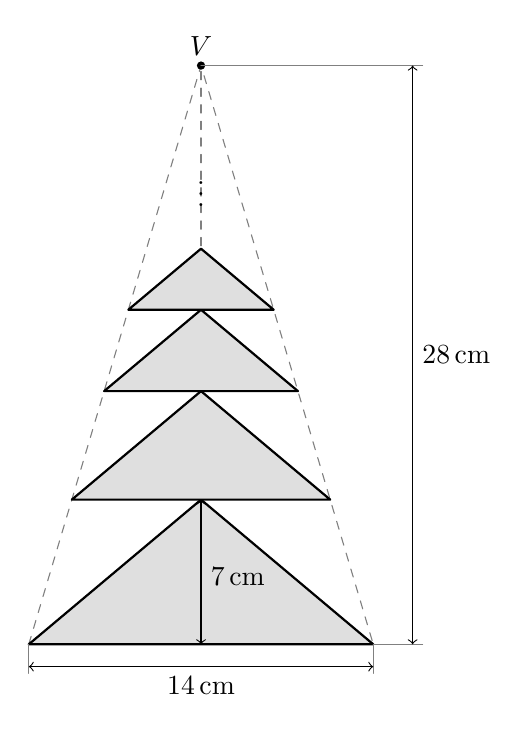
\begin{tikzpicture}[x=1.25cm,y=1.05cm,line join=round,line cap=round]
            % Střed stejnolehlosti a obal celé nekonečné soustavy
            \coordinate (V) at (0,7);
            \coordinate (A1) at (-1.75,0);
            \coordinate (B1) at ( 1.75,0);

            \draw[dashed, gray] (A1)--(V)--(B1);
            \draw[dashed, gray] (0,0)--(V);

            % k = 3/4. Každý další trojúhelník je obrazem předchozího
            % ve stejnolehlosti se středem V.
            % 1. trojúhelník: h_1 = 1.75 (odpovídá 7 cm)
            \filldraw[fill=gray!25, thick]
                (-1.75,0)--(1.75,0)--(0,1.75)--cycle;

            % 2. trojúhelník
            \filldraw[fill=gray!25, thick]
                (-1.3125,1.75)--(1.3125,1.75)--(0,3.0625)--cycle;

            % 3. trojúhelník
            \filldraw[fill=gray!25, thick]
                (-0.984375,3.0625)--(0.984375,3.0625)--(0,4.046875)--cycle;

            % 4. trojúhelník
            \filldraw[fill=gray!25, thick]
                (-0.738281,4.046875)--(0.738281,4.046875)--(0,4.785156)--cycle;

            % pokračování nekonečné posloupnosti
            \node at (0,5.55) {$\vdots$};

            % střed stejnolehlosti
            \fill (V) circle (1.5pt);
            \node[above] at (V) {$V$};

            % rozměr základny 14 cm
            \draw[gray] (-1.75,0)--(-1.75,-0.35);
            \draw[gray] ( 1.75,0)--( 1.75,-0.35);
            \draw[<->] (-1.75,-0.27)--(1.75,-0.27);
            \node[below] at (0,-0.27) {$14\,\mathrm{cm}$};

            % výška největšího trojúhelníku 7 cm
            \draw[<->] (0,0)--(0,1.75);
            \node[right] at (0,0.82) {$7\,\mathrm{cm}$};

            % výška celého obrazce 28 cm
            \draw[gray] (1.75,0)--(2.25,0);
            \draw[gray] (0,7)--(2.25,7);
            \draw[<->] (2.15,0)--(2.15,7);
            \node[right] at (2.15,3.5) {$28\,\mathrm{cm}$};
        \end{tikzpicture}
    \end{center}

    Vypočítejte v $\mathrm{cm}^2$ obsah celého šedého obrazce. Ve svém řešení nejprve
    určete koeficient stejnolehlosti dvou sousedních trojúhelníků a následně využijte
    vztah mezi koeficientem podobnosti a poměrem obsahů podobných útvarů.

    \begin{flushright}
        \textit{Upraveno podle CZVV, Matematika rozšiřující, 2021, úloha 10.}
    \end{flushright}

\end{exercise}


% =========================
% ÚLOHA 19 – Matematika rozšiřující 2023: otočení čtverce
% =========================

\begin{exercise}[BONUS: Otočení čtverce a obsah průniku]

    Je dán čtverec $ABCD$ o straně délky $3\,\mathrm{cm}$. V otočení
    \[
        \mathcal{R}(A;28^\circ)
    \]
    je jeho obrazem čtverec $AB'C'D'$. Bod $X$ je průsečíkem úseček $CD$ a $B'C'$.
    Průnik obou čtverců tvoří čtyřúhelník $AB'XD$, který je osově souměrný podle přímky $AX$.

    \begin{center}
        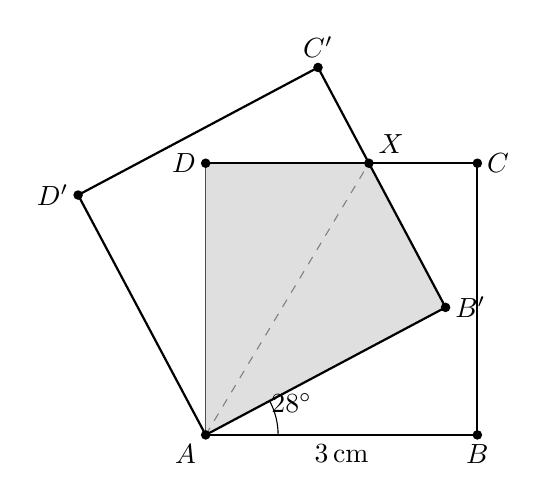
\begin{tikzpicture}[scale=1.15,line join=round]
            \coordinate (A) at (0,0);
            \coordinate (B) at (3,0);
            \coordinate (C) at (3,3);
            \coordinate (D) at (0,3);

            % původní čtverec
            \draw[thick] (A)--(B)--(C)--(D)--cycle;

            % obraz po otočení o 28 stupňů
            \coordinate (Bp) at (2.6488,1.4084);
            \coordinate (Cp) at (1.2404,4.0573);
            \coordinate (Dp) at (-1.4084,2.6488);
            \coordinate (X) at (1.8026,3);

            \fill[gray!25] (A)--(Bp)--(X)--(D)--cycle;
            \draw[thick] (A)--(Bp)--(Cp)--(Dp)--cycle;
            \draw[thick] (D)--(X);

            \draw[dashed, gray] (A)--(X);

            \fill (A) circle (1.5pt) node[below left] {$A$};
            \fill (B) circle (1.5pt) node[below] {$B$};
            \fill (C) circle (1.5pt) node[right] {$C$};
            \fill (D) circle (1.5pt) node[left] {$D$};
            \fill (Bp) circle (1.5pt) node[right] {$B'$};
            \fill (Cp) circle (1.5pt) node[above] {$C'$};
            \fill (Dp) circle (1.5pt) node[left] {$D'$};
            \fill (X) circle (1.5pt) node[above right] {$X$};

            \draw (0.8,0) arc[start angle=0,end angle=28,radius=0.8];
            \node at (0.95,0.35) {$28^\circ$};
            \node[below] at (1.5,0) {$3\,\mathrm{cm}$};
        \end{tikzpicture}
    \end{center}

    Vypočítejte obsah čtyřúhelníku $AB'XD$. Výsledek zaokrouhlete na desetiny $\mathrm{cm}^2$.

    \begin{flushright}
        \textit{CZVV, Matematika rozšiřující, 2023, úloha 19.}
    \end{flushright}

\end{exercise}

\end{document}